\section{Evaluation}
\label{sec:evaluation}

We evaluate \parikshan on two key aspects: (1). Live cloning, and (2). the debug window size.
In this section, we first look at the cloning suspend time, by evaluating it against some real-world applications, and a customized micro-benchmark.
We then evaluate debug-window sizes under different circumstances for a persistent network connection.

\subsection{How does cloning impact the performance of the production container?}
\label{sec:performance}
As explained in section \ref{sec:design}, live cloning requires a small suspend time, which has minimal impact on users.
Suspending is necessary to ensure that both containers are in the exact same system state.
Broadly, suspend time during live cloning can be divided in 4 parts: 
(1) Suspend \& Dump: time taken to pause and dump the container, 
(2) Pcopy after suspend: time required to complete rsync operation 
(3) Copy Dump File: time taken to copy an initial dump file.
(4) Undump \& Resume: time taken to resume the containers. 
To evaluate ``live cloning'', we ran a micro-benchmark of I/O operations, and evaluated live-cloning on some real-world applications running real-workloads:
%Depending on the workload of the container, different aspects of the suspend time can be impacted.
%The key to having "live" operation, is to have a short enough suspend time, so that it has minimal impact on the user.
%To understand the process better, and to see if it is viable for real-world scenario's, we ran two sets of experiments.
\begin{figure}[ht]
%{0.45\textwidth}
  \centering
%  \resizebox{\linewidth}{!}{
\begin{adjustbox}{max size={.45\textwidth}}
    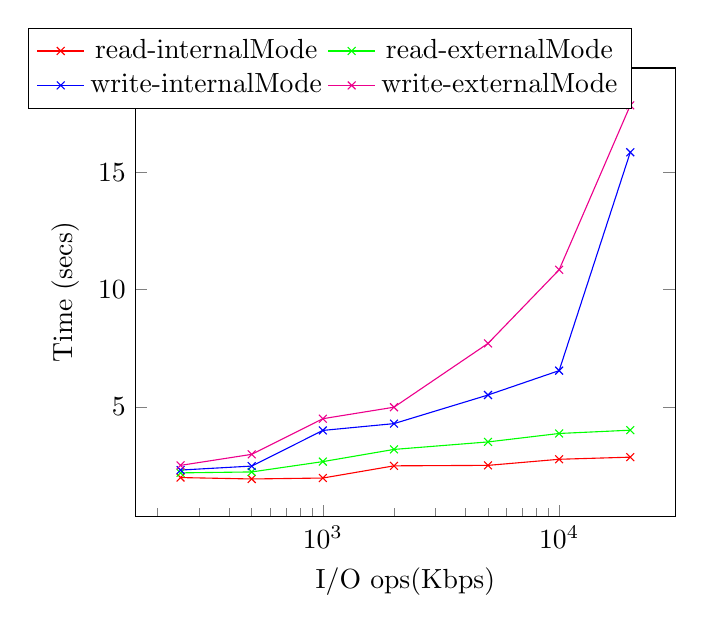
\begin{tikzpicture}
      \begin{axis}[
        xmode=log,
        legend style={at={(-0.2,1.09)},anchor=north west,legend columns=2},
        xlabel=I/O ops(Kbps),
        ylabel=Time (secs)]
        \addplot[color=red,mark=x] coordinates {
          (0,1.85)
          (250,1.99)
          (500,1.93)
          (1000,1.97)
          (2000,2.49)
          (5000,2.51)
          (10000,2.77)
          (20000,2.86)
        };
        \addlegendentry{read-internalMode}
        \addplot[color=green,mark=x] coordinates {
          (0,1.97)
          (250,2.19)
          (500,2.23)
          (1000,2.67)
          (2000,3.19)
          (5000,3.51)
          (10000,3.87)
          (20000,4.01)
        };
        \addlegendentry{read-externalMode}				
        \addplot[color=blue,mark=x] coordinates {
          (0,1.85)
          (250,2.31)
          (500,2.48)
          (1000,4.00)
          (2000,4.29)
          (5000,5.51)
          (10000,6.55)
          (20000,15.86)
        };
        \addlegendentry{write-internalMode}				
        \addplot[color=magenta,mark=x] coordinates {
          (0,1.87)
          (250,2.51)
          (500,2.98)
          (1000,4.50)
          (2000,4.99)
          (5000,7.71)
          (10000,10.85)
          (20000,17.86)
        };
        \addlegendentry{write-externalMode}
      \end{axis}
    \end{tikzpicture}
  \end{adjustbox}
%  }
  \captionsetup{justification=centering}
  \caption{Live Cloning suspend time with increasing amounts of I/O operations }
  \label{fig:fioResults}
\end{figure}


\noindent
\textbf{Micro Benchmark using I/O operations:}
%To understand the impact of cloning in further detail, we ran a micro-benchmark of an I/O application to see how well cloning scales.
%As explained earlier, the cloning process can be divided into two parts: an rsync operation which does an ``pre-copy'' of the VM, and a follow-up rsync operation while the target container is suspended, to make sure that both the production and test containers have the exact same state.
%The idea is to reduce the time taken to suspend the production container, so that it has minimal impact on the user.
The main factor that impacts suspend time is the number of ``dirty pages'' in the suspend phase, which have not been copied over in the pre-copy rsync operation (see section~\ref{sec:CloneManager}).
To understand this better, we use fio (flexible I/O tool for Linux)~\cite{fio}, to gradually increase the number of I/O operations while doing live cloning.
Fio reads or writes random values in a file with a rate controlled I/O bandwidth as specified by the user. 
The suspend time is observed by instrumentation within the cloning script, which reports time taken by each of the suspend processes.
Additionally, we ensure that the I/O job being processed by fio is long enough to last through the entire cloning process.

We found that in comparison to write, read operations have a much smaller impact on suspend time of live cloning.
This can be attributed to the increase of ``dirty pages'' in write operations, whereas for read, the disk image remains largely the same.
We also found, that internal mode is much faster than external mode, as both the production and debug-container are hosted in the same physical device.
We believe, that for higher I/O operations, with a large amount of ``dirty-pages'', network bandwidth becomes a bottleneck: leading to longer suspend times.
Overall, the internal mode is able to manage write operation up-to 10 mbps, with a total suspend-time of approx 5 seconds.
Whereas, the external mode is only able to manage upto 5-6 mbps, for a 5 sec suspend time.

%This in turn depends on I/O operations happening in the container.
%Naturally, write operations, and in memory pages in the container while cloning the container, will increase the number of dirty pages, and increase the time of the suspend operation.
%Here we also compare the performance of cloning in the internal mode vs the external mode, while showing the time taken in various stages of cloning.
%While for lower I/O operations, the performance of both were similar, as we go higher, the external mode which uses the network to transfer the dirty pages during the cloning operations becomes a bottleneck. 
%We also observed that the majority of the time is spent in pcopy after suspend, which is doing the copy of the dirty bits after suspend, especially for higher I/O's the other operations become negligible in comparison.
%For relatively lower I/O operations, "live cloning" takes only a few seconds (~2/3 secs) and is not disruptive to application clients (there is no loss of service visible). 
%However, in high I/O intensive workloads, the amount of time taken to clone can go up exponentially, and will lead to dropping of requests.
%In such cases, we did observe a few retries and in HTTP but no timeouts, naturally the performance of the server did suffer. 

\begin{figure}[ht]
  \centering
\begin{adjustbox}{max size={.45\textwidth}}
    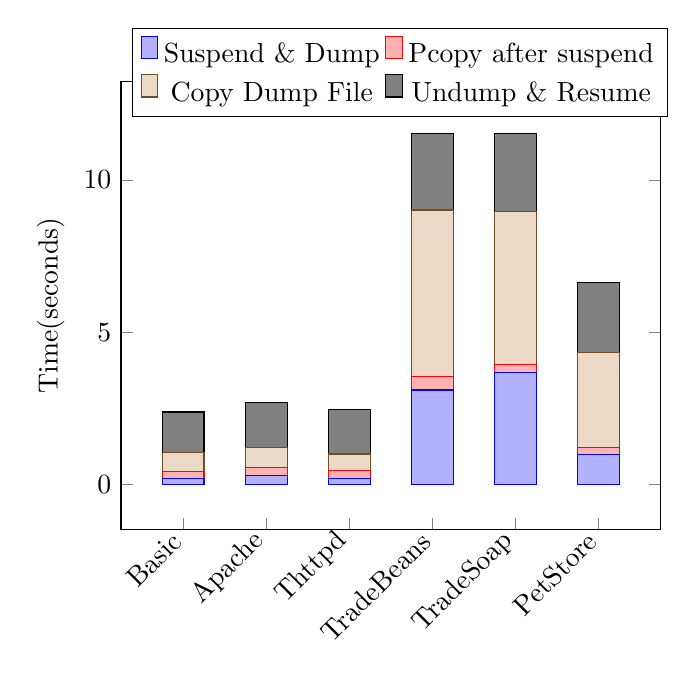
\begin{tikzpicture}
      \begin{axis}[
        ybar stacked,
        bar width=15pt,
        %	nodes near coords,
        enlargelimits=0.15,
        legend style={at={(0.02,1.12)},anchor=north west,legend columns=2},
        ylabel={Time(seconds)},
        symbolic x coords={Basic, Apache, Thttpd, TradeBeans, TradeSoap, 
          PetStore},
        xtick=data,
        x tick label style={rotate=45,anchor=east},
        ]
        \addplot+[ybar] plot coordinates {(Basic,0.21) (Apache,0.30) (Thttpd,0.21) (TradeBeans,3.10) (TradeSoap,3.68) (PetStore,0.97) };
        \addplot+[ybar] plot coordinates {(Basic,0.22) (Apache,0.27) (Thttpd,0.26) (TradeBeans,0.44) (TradeSoap,0.25) (PetStore,0.24) };
        \addplot+[ybar] plot coordinates {(Basic,0.62) (Apache,0.64) (Thttpd,0.53) (TradeBeans,5.47) (TradeSoap,5.03) (PetStore,3.11) };
        \addplot+[ybar] plot coordinates {(Basic,1.33) (Apache,1.47) (Thttpd,1.46) (TradeBeans,2.51) (TradeSoap,2.57) (PetStore,2.32) };
        \addlegendentry{\strut Suspend \& Dump}
        \addlegendentry{\strut Pcopy after suspend}
        \addlegendentry{\strut Copy Dump File}
        \addlegendentry{\strut Undump \& Resume}
        %	\legend{\strut Suspend + Dump, \strut Pcopy after suspend, \strut Copy Dump File, \strut Undump and Resume}
      \end{axis}
    \end{tikzpicture}
  \end{adjustbox}
  %\captionsetup{justification=centering}
  \caption{Suspend time for live cloning, when running a representative benchmark}
  \label{fig:stats}
\end{figure}



%\begin{figure*}[ht]
%\centering
%\begin{minipage}[b]{0.45\textwidth}
%\end{minipage}
%\quad
%\begin{minipage}[b]{0.45\textwidth}
%\end{minipage}
%\end{figure*}

\noindent
\textbf{Real-World application, and workloads:}
%To evaluate the suspend time in real-world scenarios, we tested our cloning operation on real-world applications, running a realistic workload.
In figure~\ref{fig:stats}, we show the suspend times for five well known applications. 
%both internal and external mode while comparing it with a production container, that is idle vs. a container which is running an apache hog benchmark \cite{httperf} on it. 
For Apache and thttpd, which are web-servers, we ran the httperf~\cite{httperf} hog benchmark. 
The hog benchmark tries to compute max throughput of the web-server, by sending a large number of concurrent requests.
Tradebeans and Tradesoap are both part of the dacapo~\cite{dacapo} benchmark ``DayTrader'' application.
These are realistic workloads, which run on a multi-tier trading application provided by IBM. 
PetStore~\cite{petstore} is a well known J2EE reference application. 
We deployed PetStore in a 3-tier system with JBoss, MySQL and Apache servers.
Here we cloned the app-server, and the input workload was a random set of transactions which were repeated for the duration of the cloning process.
%For MySQL we ran a similar workload with some read and write queries to test how well our cloning operation performs.
We found that for hog benchmarks, the container suspend time was 2-3 seconds.
However, for heavy workloads in more memory intensive application servers such as PetStore, DayTrader, the total suspend time was higher (6-12 seconds).
We found that we did not experience any timeouts or errors for the requests in the workload\footnote{In case of packet drops, requests are resent both at the TCP layer, and the application layer. This slows down the requests for the user, but does not drop them}.
However, this did slowdown requests in the workload. 
This confirmed our hypothesis that short suspend times are largely not visible/have minimal performance impact to the user, as they are within the time out range of most applications.
Further a clean network migration process ensures that connections are not dropped, and are executed successfully.



Live cloning can be viewed as an amortized cost paid upfront, instead of recording overhead throughout the execution.
For our future work, we aim to reduce suspend time, rate-limiting of incoming requests in the proxy, or copy-on-write mechanisms between the production container and the clone.
%Other approaches include triggering page fault for the dirty bits which were not copied over.
%This is a similar to a copy-on-write method, that could possibly reduce our suspend time.
%In the interest of time, we have not explored faster means of live cloning, but aim to do so in our future work.
%However, it would impact, the overall performance of both systems as it would do the rsync operation for a much longer time-period.

\subsection{Debug Window Size}
\label{sec:timewindowPerformance}


\begin{table}[ht]
	\centering
	\begin{tabular}{|c|r|r|r|}
		\hline
		{\bf \begin{tabular}[c]{@{}c@{}}Input \\ Rate\end{tabular}} & \multicolumn{1}{c|}{{\bf \begin{tabular}[c]{@{}c@{}}Debug \\ Window\end{tabular}}} & \multicolumn{1}{c|}{{\bf \begin{tabular}[c]{@{}c@{}}Pipe \\ Size\end{tabular}}} & \multicolumn{1}{c|}{{\bf \begin{tabular}[c]{@{}c@{}}Slow- \\ down\end{tabular}}} \\ \hline
		530 bps, 27 rq/s                                            & $\infinity$                                                                                     & 4096                                                                            & 1.8x                                                                             \\ \hline
		530 bps, 27 rq/s                                            & 8 sec                                                                              & 4096                                                                            & 3x                                                                               \\ \hline
		530 bps, 27 rq/s                                            & 72 sec                                                                             & 16384                                                                           & 3x                                                                               \\ \hline
		Poisson, $\lambda$ = 17 rq/s                                        & 16 sec                                                                             & 4096                                                                            & 8x                                                                               \\ \hline
		Poisson, $\lambda$ = 17 rq/s                                        & 18 sec                                                                             & 4096                                                                            & 5x                                                                               \\ \hline
		Poisson, $\lambda$ = 17 rq/s                                        & $\infinity$                                                                                     & 65536                                                                           & 3.2x                                                                             \\ \hline
		Poisson, $\lambda$ = 17 rq/s                                        & 376 sec                                                                            & 16384                                                                           & 3.2x                                                                             \\ \hline
	\end{tabular}
	%\captionsetup{justification=centering}
	\caption{Approximate debug window sizes for a MySQL request workload}
	\label{table:timewindow}
\end{table}

\noindent
\textbf{Experimental Results:} We call the time taken to reach a buffer overflow the ``debug-window'' for the debug-container.
As explained earlier (see section \ref{sec:window}), the size of this debug-window depends on the overhead of the ``instrumentation'', the incoming workload distribution, and the size of the buffer.
To evaluate the approximate size of the debug-window, we sent requests to both a production and debug MySQL container via our network duplicator.
Each workload ran for about 7 minutes (10,000 ``select * from table'' queries), with varying request workloads.
We also profiled the server, and found that is able to process a max of 27 req/s\footnote{Not the same as bandwidth, 27 req/s is the maximum rate of sequential requests MySQL server is able to handle for a user session} in a single user connect session. 
For each of our experiments we vary the buffer sizes to get an idea of debug-window. 
Additionally, we generated a slowdown by first modeling the time taken by MySQL to process requests (27 req/s or 17req/s), and then putting an approximate sleep in the request handler.

Initially, we created a connection, and sent requests at the maximum request rate the server was able to handle (27 req/s).
We found that for overheads up-to 1.8x (approx) we experienced no buffer overflows.
% most function tracing and profiling tools generally have an overhead of 1-1.5x for lower granularity and 2x for higher granularity tracing.
For higher overheads the debug window rapidly decreased, primarily dependent on buffer-size, request size, and slowdown.

Next, we mimic user behavior, to generate a realistic workload.
We send packets using a poisson process with an average request rate of 17 requests per second to our proxy. 
This varies the inter-request arrival time, and let's the cloned debug-container catch up with the production container during idle time-periods in between request bursts.
We observed, that compared to earlier experiments, there was more slack in the system. 
This meant that our system was able to tolerate a much higher overhead (3.2x) with no buffer overflows.


\begin{figure}[ht]
	%{0.45\textwidth}
	\centering
	%  \resizebox{\linewidth}{!}{
	\begin{adjustbox}{max size={.45\textwidth}}
		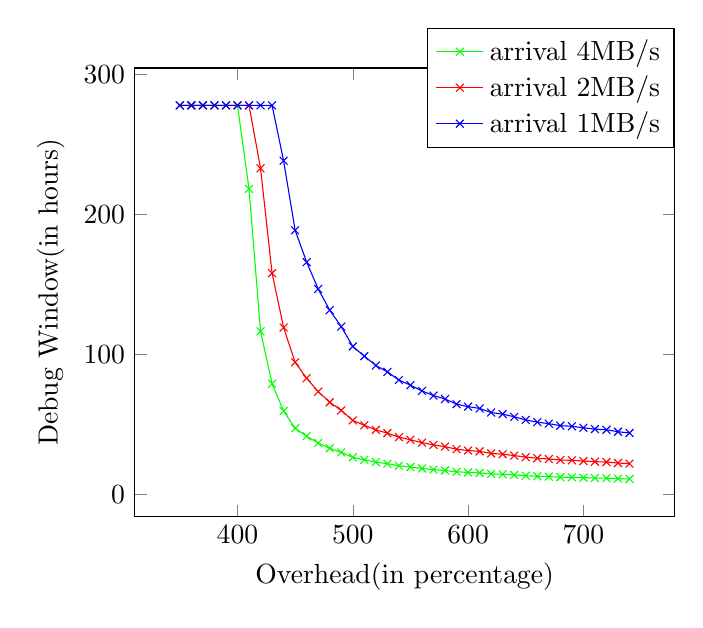
\begin{tikzpicture}
		\begin{axis}[
		%xmode=log,
		legend style={at={(1,1.09)},anchor=north east,legend columns=1},
		xlabel=Overhead(in percentage),
		ylabel=Debug Window(in hours)]
		\addplot[color=green,mark=x] coordinates {
			(350,277.7778028)
			(360,277.7778306)
			(370,277.7777806)
			(380,277.7777806)
			(390,277.777875)
			(400,277.7777972)
			(410,218.0984611)
			(420,116.3991028)
			(430,78.9657)
			(440,59.55381111)
			(450,47.147775)
			(460,41.446375)
			(470,36.65794167)
			(480,32.87560278)
			(490,29.95016111)
			(500,26.40129444)
			(510,24.66028333)
			(520,23.00362222)
			(530,21.85588056)
			(540,20.40405)
			(550,19.48659444)
			(560,18.45943611)
			(570,17.63081111)
			(580,17.01690833)
			(590,16.09901389)
			(600,15.65028056)
			(610,15.33356944)
			(620,14.601075)
			(630,14.32908611)
			(640,13.83495833)
			(650,13.29390556)
			(660,12.88229722)
			(670,12.61861944)
			(680,12.25779722)
			(690,12.14353889)
			(700,11.8762)
			(710,11.64855)
			(720,11.52348611)
			(730,11.17581111)
			(740,10.95483889)
		};
		\addlegendentry{arrival 4MB/s}
		\addplot[color=red,mark=x] coordinates {
			(350,277.7778361)
			(360,277.7777917)
			(370,277.7778389)
			(380,277.7778222)
			(390,277.7777806)
			(400,277.7778056)
			(410,277.7777778)
			(420,232.7982083)
			(430,157.9314)
			(440,119.1076194)
			(450,94.29555)
			(460,82.89275)
			(470,73.31588611)
			(480,65.75120278)
			(490,59.90032222)
			(500,52.80259167)
			(510,49.32056944)
			(520,46.00724722)
			(530,43.71176389)
			(540,40.80809722)
			(550,38.97319167)
			(560,36.91887222)
			(570,35.26162222)
			(580,34.03381667)
			(590,32.19803056)
			(600,31.30056389)
			(610,30.66714167)
			(620,29.20215)
			(630,28.65817222)
			(640,27.66991667)
			(650,26.58781389)
			(660,25.76459444)
			(670,25.23723611)
			(680,24.51559722)
			(690,24.28707778)
			(700,23.75239722)
			(710,23.2971)
			(720,23.046975)
			(730,22.35162222)
			(740,21.909675)
		};
		\addlegendentry{arrival 2MB/s}				
		\addplot[color=blue,mark=x] coordinates {
			(350,277.7778694)
			(360,277.7777944)
			(370,277.7779611)
			(380,277.7778389)
			(390,277.7777889)
			(400,277.7779139)
			(410,277.7778056)
			(420,277.7778167)
			(430,277.777875)
			(440,238.2152389)
			(450,188.5911)
			(460,165.7855028)
			(470,146.6317694)
			(480,131.5024056)
			(490,119.8006444)
			(500,105.6051806)
			(510,98.64113611)
			(520,92.01449444)
			(530,87.42352778)
			(540,81.61619722)
			(550,77.94638056)
			(560,73.83774444)
			(570,70.52324444)
			(580,68.06763333)
			(590,64.39605833)
			(600,62.60112778)
			(610,61.33428056)
			(620,58.40430278)
			(630,57.31634722)
			(640,55.33983056)
			(650,53.175625)
			(660,51.52919167)
			(670,50.474475)
			(680,49.03119167)
			(690,48.57415278)
			(700,47.50479722)
			(710,46.59420278)
			(720,46.09394722)
			(730,44.70324722)
			(740,43.81935)
		};
		\addlegendentry{arrival 1MB/s}				
		\end{axis}
		\end{tikzpicture}
	\end{adjustbox}
	%  }
	%\captionsetup{justification=centering}
	\caption{Simulation results for debug-window size. Each series has a constant arrival rate, and the buffer is kept at 64GB.}
	\label{fig:debugSim}
\end{figure}

\noindent
\textbf{Simulation Results:} 
Overall it was difficult to observe systematic behavior in a live system to understand the decay rate of the debug-window.
In our next set of experiments, we simulate packet arrival and service processing for a buffered queue in SOA applications. 
We use a discrete event simulation based on an M\/M\/1 queue, which is a  classic queuing model based on kendall's notation~\cite{kendall1953}, and is often used to model SOA applications with a single buffer based queue.
Essentially, we are sending and processing requests based on a poisson distribution with a finite buffer capacity.
%As discussed earlier, there are three parameters which can impact the time period of the debug-window: (1) arrival rate ($\lambda$), (2) service processing time ($\mu$), and (3) Buffer Size.
In our simulations (see Figure~\ref{fig:debugSim}), we kept a constant buffer size of 64GB, and iteratively increased the overhead of instrumentation, thereby decreasing the service processing time.
Each series (set of experiment), starts with an arrival rate approximately 5 times less than the service processing time. 
This means that at 400\% overhead, the system would be running at full capacity (for stable systems SOA applications generally operate at much less than system capacity).
Each simulation instance was run for 1000000 seconds or 277.7 hours.
We gradually increased the instrumentation by 10\% each time, and observed the \textit{hitting-time} of the buffer (time it takes for the buffer to overflow for the first time).
As shown there is no buffer overflow in any of the simulations until the overhead reaches around 420-470\%, beyond this the debug-window decreases exponentially.
Since beyond 400\% overhead, the system is over-capacity, the queue will start filling up fairly quickly. 
This clarifies the behavior we observed in our experiments, where for lower overheads (1.8-3.2x) we did not observe any overflow, but beyond a certain point we observed that the buffer would overflow fairly quickly.
Also as shown in the system, since the buffer size is significantly larger than the packet arrival rate, it takes some time for the buffer to overflow (several hours).
We believe that while most systems will run significantly under capacity, large buffer sizes can ensure that our debug-container may be able to handle short bursts in the workload.
However, a system running continuously at capacity is unlikely to tolerate significant instrumentation overhead.
For more details regarding queuing theory models and our detailed simulations, please have a look at our extended tech-report tech-report~\cite{parikshanQueue}.

\begin{tcolorbox}[breakable, enhanced]
		To answer \textbf{RQ2}, we found that the debug-container can stay in a stable state without any buffer overflows as long as the instrumentation does not cause the service times to become less than the request arrival rate . Furthermore, a large buffer will allow handling of short bursts in the workload until the system returns back to a stable state. 
\end{tcolorbox}

%The initial ratio between the arrival rate to the service processing rate is kept as 1:5. Hence, at 400\% overhead, the debug-container's arrival rate will be the same as the service processing rate.


\iffalse
\begin{table}[ht]
\begin{centering}
\begin{tabular}{|c|c|c|c|}
\hline
\begin{tabular}[c]{@{}c@{}}\textbf{Input} \\ \textbf{Rate}\end{tabular} & \begin{tabular}[c]{@{}c@{}}\textbf{Debug}\\ \textbf{Window}\end{tabular} & \begin{tabular}[c]{@{}c@{}}\textbf{Pipe}\\ \textbf{Size}\end{tabular} & \begin{tabular}[c]{@{}c@{}}\textbf{Slow-}\\ \textbf{down}\end{tabular}\\ \hline
530 bps, 27 rq/s                                      & $\infinity$                                                    & 4096                                                & 1.8x                      \\ \hline
530 bps, 27 rq/s                                      & 8 sec                                                  & 4096                                                & 3x                        \\ \hline
530 bps, 27 rq/s                                      & 72 sec                                                 & 16384                                               & 3x                        \\ \hline
Poisson, $\lambda$ = 17 rq/s                               & 16 sec                                                 & 4096                                                & 8x                        \\ \hline
Poisson, $\lambda$ = 17 rq/s                               & 18 sec                                                 & 4096                                                & 5x                      \\ \hline
Poisson, $\lambda$ = 17 rq/s                               & $\infinity$                                                    & 65536                                               & 3.2x \\ \hline
Poisson, $\lambda$ = 17 rq/s                               & 376 sec                                                & 16384                                               & 3.2x \\ \hline
\end{tabular}
\captionsetup{justification=centering}
\caption{Approximate debug window sizes for a MySQL request workload}
\label{table:timewindow}
\end{centering}
\end{table}
\fi


%The buffer size is configurable and for most of our case studies we kept it at 1MB.
%Hence, this is a configuration parameter that depends on the desired window size and the workload.
%We also tried a gaussian request distribution with request interarrival time being randomized to exhibhit a bursty behavior with high utilization. 
%We found that 
 
%In this section we evaluate the testing window size using varying amounts of instrumentation, and the workload.
%For the purpose of this evaluation, we keep a fixed buffer size. 
%First we use a controlled workload rate, and gradually increase the overhead, then we use another scenario, where we keep the try to keep the same overhead, and try to increase the workload.
%We also use real-world network packet capture data, to simulate a realistic workload and gradually increase the overhead there

%\texttt{Nipun's note: This section still needs to be completed, I'm finishing up some of the results, before I can generate the charts}


\iffalse
\subsection{Overhead while Running tests}
\label{sec:overhead}

One of the most important goals of using \parikshan is to allow debugging without having any overhead on the actual application.
In this section we verify that this goal of \parikshan holds true i.e. debugging in the sandbox-container, does not effect the performance container. 
To understand the effect we ran some tests on our cloned container, with an independent CPU hog (infinite while loop with sleep) running within the test.
We gradually increased the amount of CPU being used by the CPU hog and found that while in the external mode there is no effect on the performance of the production container, in the internal mode at higher CPU hog percentages, the throughput of the production container is reduced.
This was an expected result, as the production container and debug-container time share resources on the same machine, whereas in the external mode, they are completely isolated.
However, it is to be noted, that most debugging scenarios are unlikely to be CPU hogs, and if resource management in the container level is done properly, the containers in the internal-mode can be largely isolated from each other.
\fi


\iffalse
In this section we present the evaluation of \parikshan. 
The key questions facing us were:
\begin{itemize}
%  \item How can \parikshan be used in the real world? 
%  \item Does the test container faithfully represent the execution and the state of the production container? 
   \item How does cloning the container effect the performance of the production container?
   \item How long of a testing-window do we have? 
   \item How does running tests in the debug-container effect the performance of the production container?
\end{itemize}
In order to answer these questions, we separated our evaluation in looking at two different stages: cloning stage, time-window analysis.

\begin{table*}[ht]
  \centering
    \begin{tabular}{ | p{4cm} | l | l | l | l | l | l | l | l | l |}
    \hline
    \textbf{Modes} & \multicolumn{3}{|c|}{\textbf{Internal Mode}} & \multicolumn{3}{|c|}{\textbf{External Mode}} & \multicolumn{3}{|c|}{\textbf{Google Compute}}\\\hline
    \textbf{ } & \textbf{Cl} & \textbf{Hog} & \textbf{Hog+Cl} & \textbf{Cl} & \textbf{Hog} & \textbf{Hog+Cl} & \textbf{Cl} & \textbf{Hog} & \textbf{Hog+Cl} \\ \hline
    \hline
    \textbf{Throughput} & -- & 1691.0 req/s & 1509 req/s & -- & 712 & 625 & -- & 510 & 450\\ \hline
    \hline
    \textbf{Suspend + Dump} & 0.49 & -- & 0.46 & 0.10 & -- & 0.10 & 0.00 & 0.00 & 0.00\\ \hline
    \textbf{Pcopy after suspend} & 0.22 & -- & 0.27 & 0.44 & -- & 0.39 & 0.00 & 0.00 & 0.00\\ \hline
    \textbf{Copy Dump File} & 0.62 &  -- & 0.64 & 0.28 & -- & 0.31 & 0.67 & 0.00 & 0.00\\ \hline
    \textbf{Undump and Resume} & 1.33 &  -- & 1.53 & 0.84 & -- & 1.03 & 0.00 & 0.00 & 0.00\\ \hline 
    %\textbf{--------------} & --- & --- & --- & --- & --- & --- & --- & --- & --- \\ 
    \hline
    \textbf{Total Suspend Time} & 2.66 &  -- & 2.91 & 1.67 & -- & 1.83 & 0.00 & 0.00 & 0.00\\ \hline
    \end{tabular}
    \captionsetup{justification=centering}
	\caption{Performance of httpd throughput, and cloning time in external vs internal vs google compute modes}
	\label{table:clonePerf}
\end{table*}
\fi


\iffalse
The first column gives the average performance of the cloning operation without any hog operation running on it.  
An idle or a container with minimal processing is cloned relatively fast ~ 2.66 seconds on the idle container. 
We then tried to run an apache hog to make a baseline of apache's performance without cloning, and found that a simple page fetch gave us a throughput of 1691 req/s (internal mode), and then we tried to do cloning of the same container while running the hog. and found negligible change in the cloning performance.
The key thing to note in these experiments for all 3 modes, was that we \textbf{did not have any connection failure or connection refused, and only a slight decline in the throughput during the cloning operation}. 
Naturally, at the application layer, the tcp packet drops are hidden as packet resends from within tcp protocol hides the performance impact.
To further investigate the tcp packet dropping, we ran an iperf\cite{iperf}( a tool to measure tcp benchmark) server while cloning the production container. 
We were indeed able to observe packet dropping for about 2 seconds in the iperf client, however, the important point to note is that there were no requests dropped for the application while doing cloning. 


\begin{figure*}[t]
	\begin{center}
		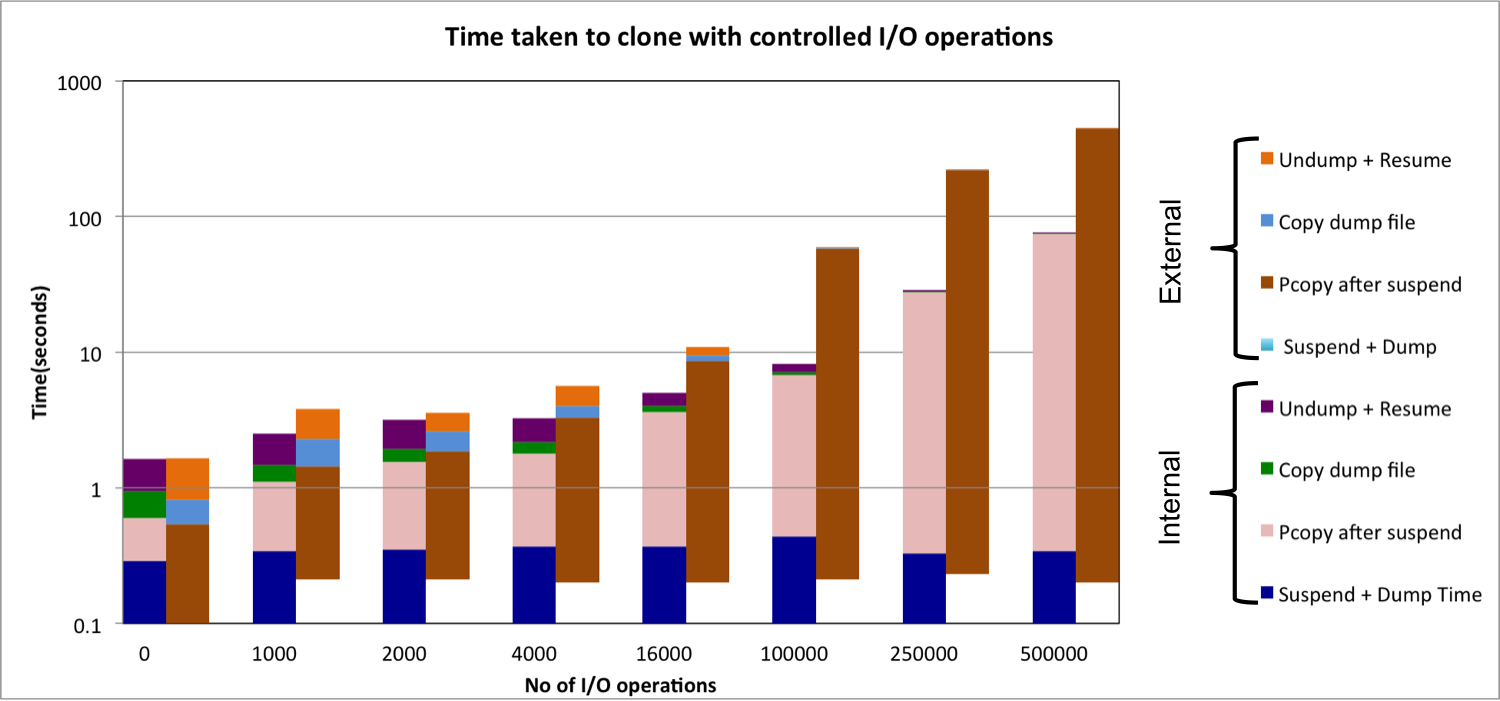
\includegraphics[width=1\textwidth]{figs/fioResult.png}
		\caption{Comparison between cloning between the internal vs external mode, while continuously increasing the file write operations to disk}
		\label{fig:fioResults}
	\end{center}
\end{figure*}
\fi
